\documentclass[1p]{elsarticle_modified}
%\bibliographystyle{elsarticle-num}

%\usepackage[colorlinks]{hyperref}
%\usepackage{abbrmath_seonhwa} %\Abb, \Ascr, \Acal ,\Abf, \Afrak
\usepackage{amsfonts}
\usepackage{amssymb}
\usepackage{amsmath}
\usepackage{amsthm}
\usepackage{scalefnt}
\usepackage{amsbsy}
\usepackage{kotex}
\usepackage{caption}
\usepackage{subfig}
\usepackage{color}
\usepackage{graphicx}
\usepackage{xcolor} %% white, black, red, green, blue, cyan, magenta, yellow
\usepackage{float}
\usepackage{setspace}
\usepackage{hyperref}

\usepackage{tikz}
\usetikzlibrary{arrows}

\usepackage{multirow}
\usepackage{array} % fixed length table
\usepackage{hhline}

%%%%%%%%%%%%%%%%%%%%%
\makeatletter
\renewcommand*\env@matrix[1][\arraystretch]{%
	\edef\arraystretch{#1}%
	\hskip -\arraycolsep
	\let\@ifnextchar\new@ifnextchar
	\array{*\c@MaxMatrixCols c}}
\makeatother %https://tex.stackexchange.com/questions/14071/how-can-i-increase-the-line-spacing-in-a-matrix
%%%%%%%%%%%%%%%

\usepackage[normalem]{ulem}

\newcommand{\msout}[1]{\ifmmode\text{\sout{\ensuremath{#1}}}\else\sout{#1}\fi}
%SOURCE: \msout is \stkout macro in https://tex.stackexchange.com/questions/20609/strikeout-in-math-mode

\newcommand{\cancel}[1]{
	\ifmmode
	{\color{red}\msout{#1}}
	\else
	{\color{red}\sout{#1}}
	\fi
}

\newcommand{\add}[1]{
	{\color{blue}\uwave{#1}}
}

\newcommand{\replace}[2]{
	\ifmmode
	{\color{red}\msout{#1}}{\color{blue}\uwave{#2}}
	\else
	{\color{red}\sout{#1}}{\color{blue}\uwave{#2}}
	\fi
}

\newcommand{\Sol}{\mathcal{S}} %segment
\newcommand{\D}{D} %diagram
\newcommand{\A}{\mathcal{A}} %arc


%%%%%%%%%%%%%%%%%%%%%%%%%%%%%5 test

\def\sl{\operatorname{\textup{SL}}(2,\Cbb)}
\def\psl{\operatorname{\textup{PSL}}(2,\Cbb)}
\def\quan{\mkern 1mu \triangleright \mkern 1mu}

\theoremstyle{definition}
\newtheorem{thm}{Theorem}[section]
\newtheorem{prop}[thm]{Proposition}
\newtheorem{lem}[thm]{Lemma}
\newtheorem{ques}[thm]{Question}
\newtheorem{cor}[thm]{Corollary}
\newtheorem{defn}[thm]{Definition}
\newtheorem{exam}[thm]{Example}
\newtheorem{rmk}[thm]{Remark}
\newtheorem{alg}[thm]{Algorithm}

\newcommand{\I}{\sqrt{-1}}
\begin{document}

%\begin{frontmatter}
%
%\title{Boundary parabolic representations of knots up to 8 crossings}
%
%%% Group authors per affiliation:
%\author{Yunhi Cho} 
%\address{Department of Mathematics, University of Seoul, Seoul, Korea}
%\ead{yhcho@uos.ac.kr}
%
%
%\author{Seonhwa Kim} %\fnref{s_kim}}
%\address{Center for Geometry and Physics, Institute for Basic Science, Pohang, 37673, Korea}
%\ead{ryeona17@ibs.re.kr}
%
%\author{Hyuk Kim}
%\address{Department of Mathematical Sciences, Seoul National University, Seoul 08826, Korea}
%\ead{hyukkim@snu.ac.kr}
%
%\author{Seokbeom Yoon}
%\address{Department of Mathematical Sciences, Seoul National University, Seoul, 08826,  Korea}
%\ead{sbyoon15@snu.ac.kr}
%
%\begin{abstract}
%We find all boundary parabolic representation of knots up to 8 crossings.
%
%\end{abstract}
%\begin{keyword}
%    \MSC[2010] 57M25 
%\end{keyword}
%
%\end{frontmatter}

%\linenumbers
%\tableofcontents
%
\newcommand\colored[1]{\textcolor{white}{\rule[-0.35ex]{0.8em}{1.4ex}}\kern-0.8em\color{red} #1}%
%\newcommand\colored[1]{\textcolor{white}{ #1}\kern-2.17ex	\textcolor{white}{ #1}\kern-1.81ex	\textcolor{white}{ #1}\kern-2.15ex\color{red}#1	}

{\Large $\underline{12n_{0586}~(K12n_{0586})}$}

\setlength{\tabcolsep}{10pt}
\renewcommand{\arraystretch}{1.6}
\vspace{1cm}\begin{tabular}{m{100pt}>{\centering\arraybackslash}m{274pt}}
\multirow{5}{120pt}{
	\centering
	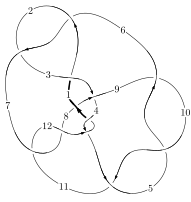
\includegraphics[width=112pt]{../../../GIT/diagram.site/Diagrams/png/2675_12n_0586.png}\\
\ \ \ A knot diagram\footnotemark}&
\allowdisplaybreaks
\textbf{Linearized knot diagam} \\
\cline{2-2}
 &
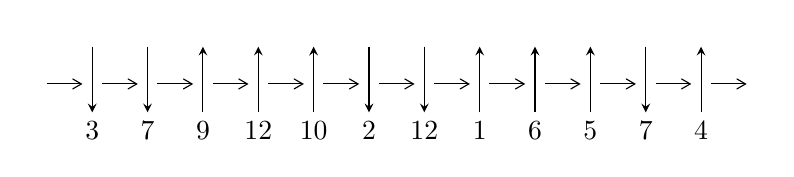
\begin{tikzpicture}[x=20pt, y=17pt]
	% nodes
	\node (C0) at (0, 0) {};
	\node (C1) at (1, 0) {};
	\node (C1U) at (1, +1) {};
	\node (C1D) at (1, -1) {3};

	\node (C2) at (2, 0) {};
	\node (C2U) at (2, +1) {};
	\node (C2D) at (2, -1) {7};

	\node (C3) at (3, 0) {};
	\node (C3U) at (3, +1) {};
	\node (C3D) at (3, -1) {9};

	\node (C4) at (4, 0) {};
	\node (C4U) at (4, +1) {};
	\node (C4D) at (4, -1) {12};

	\node (C5) at (5, 0) {};
	\node (C5U) at (5, +1) {};
	\node (C5D) at (5, -1) {10};

	\node (C6) at (6, 0) {};
	\node (C6U) at (6, +1) {};
	\node (C6D) at (6, -1) {2};

	\node (C7) at (7, 0) {};
	\node (C7U) at (7, +1) {};
	\node (C7D) at (7, -1) {12};

	\node (C8) at (8, 0) {};
	\node (C8U) at (8, +1) {};
	\node (C8D) at (8, -1) {1};

	\node (C9) at (9, 0) {};
	\node (C9U) at (9, +1) {};
	\node (C9D) at (9, -1) {6};

	\node (C10) at (10, 0) {};
	\node (C10U) at (10, +1) {};
	\node (C10D) at (10, -1) {5};

	\node (C11) at (11, 0) {};
	\node (C11U) at (11, +1) {};
	\node (C11D) at (11, -1) {7};

	\node (C12) at (12, 0) {};
	\node (C12U) at (12, +1) {};
	\node (C12D) at (12, -1) {4};
	\node (C13) at (13, 0) {};

	% arrows
	\draw[->,>={angle 60}]
	(C0) edge (C1) (C1) edge (C2) (C2) edge (C3) (C3) edge (C4) (C4) edge (C5) (C5) edge (C6) (C6) edge (C7) (C7) edge (C8) (C8) edge (C9) (C9) edge (C10) (C10) edge (C11) (C11) edge (C12) (C12) edge (C13) ;	\draw[->,>=stealth]
	(C1U) edge (C1D) (C2U) edge (C2D) (C3D) edge (C3U) (C4D) edge (C4U) (C5D) edge (C5U) (C6U) edge (C6D) (C7U) edge (C7D) (C8D) edge (C8U) (C9D) edge (C9U) (C10D) edge (C10U) (C11U) edge (C11D) (C12D) edge (C12U) ;
	\end{tikzpicture} \\
\hhline{~~} \\& 
\textbf{Solving Sequence} \\ \cline{2-2} 
 &
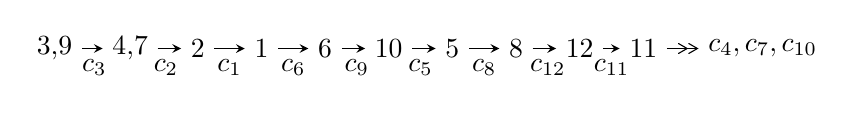
\begin{tikzpicture}[x=23pt, y=7pt]
	% node
	\node (A0) at (-1/8, 0) {3,9};
	\node (A1) at (17/16, 0) {4,7};
	\node (A2) at (17/8, 0) {2};
	\node (A3) at (25/8, 0) {1};
	\node (A4) at (33/8, 0) {6};
	\node (A5) at (41/8, 0) {10};
	\node (A6) at (49/8, 0) {5};
	\node (A7) at (57/8, 0) {8};
	\node (A8) at (65/8, 0) {12};
	\node (A9) at (73/8, 0) {11};
	\node (C1) at (1/2, -1) {$c_{3}$};
	\node (C2) at (13/8, -1) {$c_{2}$};
	\node (C3) at (21/8, -1) {$c_{1}$};
	\node (C4) at (29/8, -1) {$c_{6}$};
	\node (C5) at (37/8, -1) {$c_{9}$};
	\node (C6) at (45/8, -1) {$c_{5}$};
	\node (C7) at (53/8, -1) {$c_{8}$};
	\node (C8) at (61/8, -1) {$c_{12}$};
	\node (C9) at (69/8, -1) {$c_{11}$};
	\node (A10) at (11, 0) {$c_{4},c_{7},c_{10}$};

	% edge
	\draw[->,>=stealth]	
	(A0) edge (A1) (A1) edge (A2) (A2) edge (A3) (A3) edge (A4) (A4) edge (A5) (A5) edge (A6) (A6) edge (A7) (A7) edge (A8) (A8) edge (A9) ;
	\draw[->>,>={angle 60}]	
	(A9) edge (A10);
\end{tikzpicture} \\ 

\end{tabular} \\

\footnotetext{
The image of knot diagram is generated by the software ``\textbf{Draw programme}" developed by Andrew Bartholomew(\url{http://www.layer8.co.uk/maths/draw/index.htm\#Running-draw}), where we modified some parts for our purpose(\url{https://github.com/CATsTAILs/LinksPainter}).
}\phantom \\ \newline 
\centering \textbf{Ideals for irreducible components\footnotemark of $X_{\text{par}}$} 
 
\begin{align*}
I^u_{1}&=\langle 
5.84707\times10^{197} u^{67}-2.16837\times10^{197} u^{66}+\cdots+3.92981\times10^{199} b-1.61157\times10^{200},\\
\phantom{I^u_{1}}&\phantom{= \langle  }-5.53238\times10^{199} u^{67}-9.61476\times10^{198} u^{66}+\cdots+1.84701\times10^{201} a+1.52628\times10^{202},\\
\phantom{I^u_{1}}&\phantom{= \langle  }u^{68}+u^{67}+\cdots-106 u+47\rangle \\
I^u_{2}&=\langle 
-209 u^{17}-81 u^{16}+\cdots+310 b+36,\;-244 u^{17}+1029 u^{16}+\cdots+1550 a+3366,\\
\phantom{I^u_{2}}&\phantom{= \langle  }u^{18}+8 u^{16}+\cdots- u+1\rangle \\
\\
\end{align*}
\raggedright * 2 irreducible components of $\dim_{\mathbb{C}}=0$, with total 86 representations.\\
\footnotetext{All coefficients of polynomials are rational numbers. But the coefficients are sometimes approximated in decimal forms when there is not enough margin.}
\newpage
\renewcommand{\arraystretch}{1}
\centering \section*{I. $I^u_{1}= \langle 5.85\times10^{197} u^{67}-2.17\times10^{197} u^{66}+\cdots+3.93\times10^{199} b-1.61\times10^{200},\;-5.53\times10^{199} u^{67}-9.61\times10^{198} u^{66}+\cdots+1.85\times10^{201} a+1.53\times10^{202},\;u^{68}+u^{67}+\cdots-106 u+47 \rangle$}
\flushleft \textbf{(i) Arc colorings}\\
\begin{tabular}{m{7pt} m{180pt} m{7pt} m{180pt} }
\flushright $a_{3}=$&$\begin{pmatrix}1\\0\end{pmatrix}$ \\
\flushright $a_{9}=$&$\begin{pmatrix}0\\u\end{pmatrix}$ \\
\flushright $a_{4}=$&$\begin{pmatrix}1\\- u^2\end{pmatrix}$ \\
\flushright $a_{7}=$&$\begin{pmatrix}0.0299532 u^{67}+0.00520559 u^{66}+\cdots+50.3165 u-8.26352\\-0.0148788 u^{67}+0.00551776 u^{66}+\cdots-6.75829 u+4.10088\end{pmatrix}$ \\
\flushright $a_{2}=$&$\begin{pmatrix}-0.0362808 u^{67}-0.0242750 u^{66}+\cdots-44.0012 u+7.42020\\-0.00689572 u^{67}-0.0259460 u^{66}+\cdots+10.0543 u-4.06600\end{pmatrix}$ \\
\flushright $a_{1}=$&$\begin{pmatrix}-0.0431766 u^{67}-0.0502210 u^{66}+\cdots-33.9469 u+3.35420\\-0.00689572 u^{67}-0.0259460 u^{66}+\cdots+10.0543 u-4.06600\end{pmatrix}$ \\
\flushright $a_{6}=$&$\begin{pmatrix}-0.0624288 u^{67}-0.0963950 u^{66}+\cdots+15.2630 u-9.17122\\-0.00205894 u^{67}-0.0212165 u^{66}+\cdots+6.50316 u-1.16309\end{pmatrix}$ \\
\flushright $a_{10}=$&$\begin{pmatrix}0.0381559 u^{67}+0.0535170 u^{66}+\cdots-3.05160 u+8.01004\\-0.0347763 u^{67}-0.0318760 u^{66}+\cdots-6.01436 u+0.490177\end{pmatrix}$ \\
\flushright $a_{5}=$&$\begin{pmatrix}-0.0944015 u^{67}-0.124449 u^{66}+\cdots-6.54416 u-8.59604\\-0.00498418 u^{67}-0.00962390 u^{66}+\cdots+6.80395 u-1.39075\end{pmatrix}$ \\
\flushright $a_{8}=$&$\begin{pmatrix}0.103443 u^{67}+0.122227 u^{66}+\cdots+44.4358 u+2.42709\\-0.0284046 u^{67}+0.00567057 u^{66}+\cdots-13.2395 u+4.22413\end{pmatrix}$ \\
\flushright $a_{12}=$&$\begin{pmatrix}-0.0320963 u^{67}-0.0324433 u^{66}+\cdots-45.2838 u+7.08912\\0.00120374 u^{67}-0.0159271 u^{66}+\cdots+9.86516 u-3.75123\end{pmatrix}$ \\
\flushright $a_{11}=$&$\begin{pmatrix}-0.0569399 u^{67}-0.0655646 u^{66}+\cdots-37.3182 u-4.99682\\0.0560391 u^{67}+0.0440243 u^{66}+\cdots+22.0532 u-5.21740\end{pmatrix}$\\&\end{tabular}
\flushleft \textbf{(ii) Obstruction class $= -1$}\\~\\
\flushleft \textbf{(iii) Cusp Shapes $= -0.100434 u^{67}-0.0117449 u^{66}+\cdots-58.9561 u+13.3433$}\\~\\
\newpage\renewcommand{\arraystretch}{1}
\flushleft \textbf{(iv) u-Polynomials at the component}\newline \\
\begin{tabular}{m{50pt}|m{274pt}}
Crossings & \hspace{64pt}u-Polynomials at each crossing \\
\hline $$\begin{aligned}c_{1}\end{aligned}$$&$\begin{aligned}
&u^{68}+27 u^{67}+\cdots+475766 u+29929
\end{aligned}$\\
\hline $$\begin{aligned}c_{2},c_{6}\end{aligned}$$&$\begin{aligned}
&u^{68}- u^{67}+\cdots+4 u+173
\end{aligned}$\\
\hline $$\begin{aligned}c_{3}\end{aligned}$$&$\begin{aligned}
&u^{68}- u^{67}+\cdots+106 u+47
\end{aligned}$\\
\hline $$\begin{aligned}c_{4},c_{12}\end{aligned}$$&$\begin{aligned}
&u^{68}+3 u^{67}+\cdots+15 u+1
\end{aligned}$\\
\hline $$\begin{aligned}c_{5},c_{9},c_{10}\end{aligned}$$&$\begin{aligned}
&u^{68}- u^{67}+\cdots+257 u+49
\end{aligned}$\\
\hline $$\begin{aligned}c_{7},c_{11}\end{aligned}$$&$\begin{aligned}
&u^{68}+27 u^{66}+\cdots+1735 u+187
\end{aligned}$\\
\hline $$\begin{aligned}c_{8}\end{aligned}$$&$\begin{aligned}
&u^{68}+3 u^{67}+\cdots+4213 u+2417
\end{aligned}$\\
\hline
\end{tabular}\\~\\
\newpage\renewcommand{\arraystretch}{1}
\flushleft \textbf{(v) Riley Polynomials at the component}\newline \\
\begin{tabular}{m{50pt}|m{274pt}}
Crossings & \hspace{64pt}Riley Polynomials at each crossing \\
\hline $$\begin{aligned}c_{1}\end{aligned}$$&$\begin{aligned}
&y^{68}+25 y^{67}+\cdots+3728354922 y+895745041
\end{aligned}$\\
\hline $$\begin{aligned}c_{2},c_{6}\end{aligned}$$&$\begin{aligned}
&y^{68}-27 y^{67}+\cdots-475766 y+29929
\end{aligned}$\\
\hline $$\begin{aligned}c_{3}\end{aligned}$$&$\begin{aligned}
&y^{68}+25 y^{67}+\cdots+82858 y+2209
\end{aligned}$\\
\hline $$\begin{aligned}c_{4},c_{12}\end{aligned}$$&$\begin{aligned}
&y^{68}+19 y^{67}+\cdots-7 y+1
\end{aligned}$\\
\hline $$\begin{aligned}c_{5},c_{9},c_{10}\end{aligned}$$&$\begin{aligned}
&y^{68}+55 y^{67}+\cdots+9411 y+2401
\end{aligned}$\\
\hline $$\begin{aligned}c_{7},c_{11}\end{aligned}$$&$\begin{aligned}
&y^{68}+54 y^{67}+\cdots+2636053 y+34969
\end{aligned}$\\
\hline $$\begin{aligned}c_{8}\end{aligned}$$&$\begin{aligned}
&y^{68}-23 y^{67}+\cdots-227917187 y+5841889
\end{aligned}$\\
\hline
\end{tabular}\\~\\
\newpage\flushleft \textbf{(vi) Complex Volumes and Cusp Shapes}
$$\begin{array}{c|c|c}  
\text{Solutions to }I^u_{1}& \I (\text{vol} + \sqrt{-1}CS) & \text{Cusp shape}\\
 \hline 
\begin{aligned}
u &= -0.219883 + 1.008080 I \\
a &= \phantom{-}0.241469 + 0.085640 I \\
b &= \phantom{-}1.49707 + 0.09193 I\end{aligned}
 & -6.12896 - 5.89482 I & -5.75652 + 6.05557 I \\ \hline\begin{aligned}
u &= -0.219883 - 1.008080 I \\
a &= \phantom{-}0.241469 - 0.085640 I \\
b &= \phantom{-}1.49707 - 0.09193 I\end{aligned}
 & -6.12896 + 5.89482 I & -5.75652 - 6.05557 I \\ \hline\begin{aligned}
u &= \phantom{-}0.672615 + 0.850472 I \\
a &= -0.83876 - 1.21241 I \\
b &= -1.100020 + 0.411678 I\end{aligned}
 & -1.73558 + 5.05503 I & \phantom{-0.000000 } 0 \\ \hline\begin{aligned}
u &= \phantom{-}0.672615 - 0.850472 I \\
a &= -0.83876 + 1.21241 I \\
b &= -1.100020 - 0.411678 I\end{aligned}
 & -1.73558 - 5.05503 I & \phantom{-0.000000 } 0 \\ \hline\begin{aligned}
u &= -0.697134 + 0.586038 I \\
a &= -0.177708 + 1.159770 I \\
b &= \phantom{-}0.620030 - 1.084450 I\end{aligned}
 & \phantom{-}2.62024 - 1.78240 I & \phantom{-}2.56416 + 3.76388 I \\ \hline\begin{aligned}
u &= -0.697134 - 0.586038 I \\
a &= -0.177708 - 1.159770 I \\
b &= \phantom{-}0.620030 + 1.084450 I\end{aligned}
 & \phantom{-}2.62024 + 1.78240 I & \phantom{-}2.56416 - 3.76388 I \\ \hline\begin{aligned}
u &= \phantom{-}0.285172 + 1.071980 I \\
a &= -0.250112 - 1.333290 I \\
b &= -0.774404 + 0.244058 I\end{aligned}
 & -3.84364 + 0.87290 I & \phantom{-0.000000 } 0 \\ \hline\begin{aligned}
u &= \phantom{-}0.285172 - 1.071980 I \\
a &= -0.250112 + 1.333290 I \\
b &= -0.774404 - 0.244058 I\end{aligned}
 & -3.84364 - 0.87290 I & \phantom{-0.000000 } 0 \\ \hline\begin{aligned}
u &= \phantom{-}0.862398 + 0.778967 I \\
a &= -0.413310 - 1.002620 I \\
b &= \phantom{-}0.248323 + 0.742821 I\end{aligned}
 & -2.25225 + 2.76690 I & \phantom{-0.000000 } 0 \\ \hline\begin{aligned}
u &= \phantom{-}0.862398 - 0.778967 I \\
a &= -0.413310 + 1.002620 I \\
b &= \phantom{-}0.248323 - 0.742821 I\end{aligned}
 & -2.25225 - 2.76690 I & \phantom{-0.000000 } 0\\
 \hline 
 \end{array}$$\newpage$$\begin{array}{c|c|c}  
\text{Solutions to }I^u_{1}& \I (\text{vol} + \sqrt{-1}CS) & \text{Cusp shape}\\
 \hline 
\begin{aligned}
u &= \phantom{-}0.825035 + 0.118193 I \\
a &= -1.265070 - 0.030158 I \\
b &= \phantom{-}0.727846 - 0.338916 I\end{aligned}
 & -0.34308 + 2.06616 I & -0.45806 - 4.18693 I \\ \hline\begin{aligned}
u &= \phantom{-}0.825035 - 0.118193 I \\
a &= -1.265070 + 0.030158 I \\
b &= \phantom{-}0.727846 + 0.338916 I\end{aligned}
 & -0.34308 - 2.06616 I & -0.45806 + 4.18693 I \\ \hline\begin{aligned}
u &= -0.652354 + 0.456929 I \\
a &= \phantom{-}0.416523 - 0.539818 I \\
b &= -0.260189 + 0.688100 I\end{aligned}
 & \phantom{-}1.12611 - 0.90841 I & \phantom{-}6.23168 + 2.86305 I \\ \hline\begin{aligned}
u &= -0.652354 - 0.456929 I \\
a &= \phantom{-}0.416523 + 0.539818 I \\
b &= -0.260189 - 0.688100 I\end{aligned}
 & \phantom{-}1.12611 + 0.90841 I & \phantom{-}6.23168 - 2.86305 I \\ \hline\begin{aligned}
u &= \phantom{-}0.547303 + 1.073360 I \\
a &= -0.385360 - 1.119290 I \\
b &= -1.27680 + 0.71611 I\end{aligned}
 & -2.44164 + 6.42080 I & \phantom{-0.000000 } 0 \\ \hline\begin{aligned}
u &= \phantom{-}0.547303 - 1.073360 I \\
a &= -0.385360 + 1.119290 I \\
b &= -1.27680 - 0.71611 I\end{aligned}
 & -2.44164 - 6.42080 I & \phantom{-0.000000 } 0 \\ \hline\begin{aligned}
u &= -0.408196 + 1.150410 I \\
a &= -0.035504 - 0.295582 I \\
b &= -1.201720 + 0.270622 I\end{aligned}
 & -6.60076 + 0.55952 I & \phantom{-0.000000 } 0 \\ \hline\begin{aligned}
u &= -0.408196 - 1.150410 I \\
a &= -0.035504 + 0.295582 I \\
b &= -1.201720 - 0.270622 I\end{aligned}
 & -6.60076 - 0.55952 I & \phantom{-0.000000 } 0 \\ \hline\begin{aligned}
u &= -0.370976 + 1.165800 I \\
a &= \phantom{-}0.626431 - 0.837333 I \\
b &= \phantom{-}0.950656 + 0.634963 I\end{aligned}
 & -1.29490 - 3.01799 I & \phantom{-0.000000 } 0 \\ \hline\begin{aligned}
u &= -0.370976 - 1.165800 I \\
a &= \phantom{-}0.626431 + 0.837333 I \\
b &= \phantom{-}0.950656 - 0.634963 I\end{aligned}
 & -1.29490 + 3.01799 I & \phantom{-0.000000 } 0\\
 \hline 
 \end{array}$$\newpage$$\begin{array}{c|c|c}  
\text{Solutions to }I^u_{1}& \I (\text{vol} + \sqrt{-1}CS) & \text{Cusp shape}\\
 \hline 
\begin{aligned}
u &= \phantom{-}1.092950 + 0.590264 I \\
a &= \phantom{-}0.330797 + 0.819225 I \\
b &= -0.803251 - 0.823757 I\end{aligned}
 & \phantom{-}6.26049 - 3.07517 I & \phantom{-0.000000 } 0 \\ \hline\begin{aligned}
u &= \phantom{-}1.092950 - 0.590264 I \\
a &= \phantom{-}0.330797 - 0.819225 I \\
b &= -0.803251 + 0.823757 I\end{aligned}
 & \phantom{-}6.26049 + 3.07517 I & \phantom{-0.000000 } 0 \\ \hline\begin{aligned}
u &= -1.208810 + 0.326750 I \\
a &= \phantom{-}1.227870 - 0.540184 I \\
b &= -0.888058 + 0.281420 I\end{aligned}
 & -0.63925 - 3.06252 I & \phantom{-0.000000 } 0 \\ \hline\begin{aligned}
u &= -1.208810 - 0.326750 I \\
a &= \phantom{-}1.227870 + 0.540184 I \\
b &= -0.888058 - 0.281420 I\end{aligned}
 & -0.63925 + 3.06252 I & \phantom{-0.000000 } 0 \\ \hline\begin{aligned}
u &= \phantom{-}0.982954 + 0.811230 I \\
a &= \phantom{-}0.647738 + 1.181950 I \\
b &= \phantom{-}0.686495 - 0.648752 I\end{aligned}
 & \phantom{-}2.50618 - 3.05539 I & \phantom{-0.000000 } 0 \\ \hline\begin{aligned}
u &= \phantom{-}0.982954 - 0.811230 I \\
a &= \phantom{-}0.647738 - 1.181950 I \\
b &= \phantom{-}0.686495 + 0.648752 I\end{aligned}
 & \phantom{-}2.50618 + 3.05539 I & \phantom{-0.000000 } 0 \\ \hline\begin{aligned}
u &= \phantom{-}0.058122 + 0.694950 I \\
a &= \phantom{-}0.497793 + 0.157791 I \\
b &= \phantom{-}0.277847 + 0.724175 I\end{aligned}
 & \phantom{-}0.07404 - 1.89460 I & \phantom{-}0.12200 + 5.75647 I \\ \hline\begin{aligned}
u &= \phantom{-}0.058122 - 0.694950 I \\
a &= \phantom{-}0.497793 - 0.157791 I \\
b &= \phantom{-}0.277847 - 0.724175 I\end{aligned}
 & \phantom{-}0.07404 + 1.89460 I & \phantom{-}0.12200 - 5.75647 I \\ \hline\begin{aligned}
u &= -0.250739 + 0.644457 I \\
a &= \phantom{-}0.359250 - 0.769410 I \\
b &= -0.216911 + 1.356100 I\end{aligned}
 & \phantom{-}1.036920 + 0.367328 I & \phantom{-}0.04414 + 3.61743 I \\ \hline\begin{aligned}
u &= -0.250739 - 0.644457 I \\
a &= \phantom{-}0.359250 + 0.769410 I \\
b &= -0.216911 - 1.356100 I\end{aligned}
 & \phantom{-}1.036920 - 0.367328 I & \phantom{-}0.04414 - 3.61743 I\\
 \hline 
 \end{array}$$\newpage$$\begin{array}{c|c|c}  
\text{Solutions to }I^u_{1}& \I (\text{vol} + \sqrt{-1}CS) & \text{Cusp shape}\\
 \hline 
\begin{aligned}
u &= \phantom{-}0.272972 + 0.634333 I \\
a &= -1.06513 - 2.33502 I \\
b &= -1.243240 + 0.447834 I\end{aligned}
 & -4.27261 + 6.00177 I & -7.74759 - 4.23615 I \\ \hline\begin{aligned}
u &= \phantom{-}0.272972 - 0.634333 I \\
a &= -1.06513 + 2.33502 I \\
b &= -1.243240 - 0.447834 I\end{aligned}
 & -4.27261 - 6.00177 I & -7.74759 + 4.23615 I \\ \hline\begin{aligned}
u &= -0.002617 + 0.674324 I \\
a &= \phantom{-}1.32887 - 0.85280 I \\
b &= \phantom{-}1.049360 + 0.436998 I\end{aligned}
 & -1.81410 - 2.04263 I & \phantom{-}0.563270 - 0.027667 I \\ \hline\begin{aligned}
u &= -0.002617 - 0.674324 I \\
a &= \phantom{-}1.32887 + 0.85280 I \\
b &= \phantom{-}1.049360 - 0.436998 I\end{aligned}
 & -1.81410 + 2.04263 I & \phantom{-}0.563270 + 0.027667 I \\ \hline\begin{aligned}
u &= \phantom{-}0.953638 + 0.930205 I \\
a &= -0.061568 + 1.227830 I \\
b &= \phantom{-}1.134930 - 0.766088 I\end{aligned}
 & \phantom{-}0.91776 + 8.39173 I & \phantom{-0.000000 } 0 \\ \hline\begin{aligned}
u &= \phantom{-}0.953638 - 0.930205 I \\
a &= -0.061568 - 1.227830 I \\
b &= \phantom{-}1.134930 + 0.766088 I\end{aligned}
 & \phantom{-}0.91776 - 8.39173 I & \phantom{-0.000000 } 0 \\ \hline\begin{aligned}
u &= \phantom{-}0.831876 + 1.042200 I \\
a &= \phantom{-}0.301219 + 0.859411 I \\
b &= -0.464635 - 1.087020 I\end{aligned}
 & \phantom{-}1.73649 + 9.68261 I & \phantom{-0.000000 } 0 \\ \hline\begin{aligned}
u &= \phantom{-}0.831876 - 1.042200 I \\
a &= \phantom{-}0.301219 - 0.859411 I \\
b &= -0.464635 + 1.087020 I\end{aligned}
 & \phantom{-}1.73649 - 9.68261 I & \phantom{-0.000000 } 0 \\ \hline\begin{aligned}
u &= \phantom{-}0.603553 + 0.282503 I \\
a &= -0.778437 + 0.160505 I \\
b &= \phantom{-}0.690703 + 0.550708 I\end{aligned}
 & -0.35366 - 1.81069 I & \phantom{-}0.78941 + 4.64201 I \\ \hline\begin{aligned}
u &= \phantom{-}0.603553 - 0.282503 I \\
a &= -0.778437 - 0.160505 I \\
b &= \phantom{-}0.690703 - 0.550708 I\end{aligned}
 & -0.35366 + 1.81069 I & \phantom{-}0.78941 - 4.64201 I\\
 \hline 
 \end{array}$$\newpage$$\begin{array}{c|c|c}  
\text{Solutions to }I^u_{1}& \I (\text{vol} + \sqrt{-1}CS) & \text{Cusp shape}\\
 \hline 
\begin{aligned}
u &= -0.999379 + 0.885451 I \\
a &= -0.229036 + 1.255670 I \\
b &= -0.929485 - 0.752340 I\end{aligned}
 & \phantom{-}5.84722 - 2.80393 I & \phantom{-0.000000 } 0 \\ \hline\begin{aligned}
u &= -0.999379 - 0.885451 I \\
a &= -0.229036 - 1.255670 I \\
b &= -0.929485 + 0.752340 I\end{aligned}
 & \phantom{-}5.84722 + 2.80393 I & \phantom{-0.000000 } 0 \\ \hline\begin{aligned}
u &= -0.245626 + 1.337940 I \\
a &= -0.097385 - 1.229590 I \\
b &= \phantom{-}0.926966 + 0.720129 I\end{aligned}
 & -5.22159 - 2.81789 I & \phantom{-0.000000 } 0 \\ \hline\begin{aligned}
u &= -0.245626 - 1.337940 I \\
a &= -0.097385 + 1.229590 I \\
b &= \phantom{-}0.926966 - 0.720129 I\end{aligned}
 & -5.22159 + 2.81789 I & \phantom{-0.000000 } 0 \\ \hline\begin{aligned}
u &= -0.590766 + 1.231350 I \\
a &= -1.050480 + 0.810433 I \\
b &= -0.881595 - 0.567034 I\end{aligned}
 & \phantom{-}0.52888 - 3.31346 I & \phantom{-0.000000 } 0 \\ \hline\begin{aligned}
u &= -0.590766 - 1.231350 I \\
a &= -1.050480 - 0.810433 I \\
b &= -0.881595 + 0.567034 I\end{aligned}
 & \phantom{-}0.52888 + 3.31346 I & \phantom{-0.000000 } 0 \\ \hline\begin{aligned}
u &= -0.942984 + 1.008420 I \\
a &= -0.394979 + 0.529136 I \\
b &= \phantom{-}0.635572 - 0.849451 I\end{aligned}
 & \phantom{-}5.46665 - 4.25985 I & \phantom{-0.000000 } 0 \\ \hline\begin{aligned}
u &= -0.942984 - 1.008420 I \\
a &= -0.394979 - 0.529136 I \\
b &= \phantom{-}0.635572 + 0.849451 I\end{aligned}
 & \phantom{-}5.46665 + 4.25985 I & \phantom{-0.000000 } 0 \\ \hline\begin{aligned}
u &= -0.280602 + 0.476354 I \\
a &= \phantom{-}1.06036 + 1.78747 I \\
b &= -0.983679 - 0.799011 I\end{aligned}
 & -8.64170 - 3.14980 I & \phantom{-}7.16331 + 0.66341 I \\ \hline\begin{aligned}
u &= -0.280602 - 0.476354 I \\
a &= \phantom{-}1.06036 - 1.78747 I \\
b &= -0.983679 + 0.799011 I\end{aligned}
 & -8.64170 + 3.14980 I & \phantom{-}7.16331 - 0.66341 I\\
 \hline 
 \end{array}$$\newpage$$\begin{array}{c|c|c}  
\text{Solutions to }I^u_{1}& \I (\text{vol} + \sqrt{-1}CS) & \text{Cusp shape}\\
 \hline 
\begin{aligned}
u &= \phantom{-}0.307300 + 0.457812 I \\
a &= -3.78079 + 0.68872 I \\
b &= -0.869527 - 0.011159 I\end{aligned}
 & -0.58727 + 4.50387 I & -4.76464 - 6.42986 I \\ \hline\begin{aligned}
u &= \phantom{-}0.307300 - 0.457812 I \\
a &= -3.78079 - 0.68872 I \\
b &= -0.869527 + 0.011159 I\end{aligned}
 & -0.58727 - 4.50387 I & -4.76464 + 6.42986 I \\ \hline\begin{aligned}
u &= \phantom{-}1.02698 + 1.04640 I \\
a &= \phantom{-}0.458414 + 0.098682 I \\
b &= -0.834490 - 0.563961 I\end{aligned}
 & \phantom{-}0.685407 - 1.197810 I & \phantom{-0.000000 } 0 \\ \hline\begin{aligned}
u &= \phantom{-}1.02698 - 1.04640 I \\
a &= \phantom{-}0.458414 - 0.098682 I \\
b &= -0.834490 + 0.563961 I\end{aligned}
 & \phantom{-}0.685407 + 1.197810 I & \phantom{-0.000000 } 0 \\ \hline\begin{aligned}
u &= -0.18944 + 1.46901 I \\
a &= \phantom{-}0.488604 - 0.506368 I \\
b &= \phantom{-}0.866555 - 0.189018 I\end{aligned}
 & -12.42370 + 0.82804 I & \phantom{-0.000000 } 0 \\ \hline\begin{aligned}
u &= -0.18944 - 1.46901 I \\
a &= \phantom{-}0.488604 + 0.506368 I \\
b &= \phantom{-}0.866555 + 0.189018 I\end{aligned}
 & -12.42370 - 0.82804 I & \phantom{-0.000000 } 0 \\ \hline\begin{aligned}
u &= \phantom{-}0.81297 + 1.24271 I \\
a &= \phantom{-}0.579912 + 1.211930 I \\
b &= \phantom{-}1.045700 - 0.697944 I\end{aligned}
 & \phantom{-}4.19402 + 10.02790 I & \phantom{-0.000000 } 0 \\ \hline\begin{aligned}
u &= \phantom{-}0.81297 - 1.24271 I \\
a &= \phantom{-}0.579912 - 1.211930 I \\
b &= \phantom{-}1.045700 + 0.697944 I\end{aligned}
 & \phantom{-}4.19402 - 10.02790 I & \phantom{-0.000000 } 0 \\ \hline\begin{aligned}
u &= -1.11179 + 1.00012 I \\
a &= \phantom{-}0.06005 - 1.45837 I \\
b &= \phantom{-}1.138200 + 0.543938 I\end{aligned}
 & -4.81124 - 7.61038 I & \phantom{-0.000000 } 0 \\ \hline\begin{aligned}
u &= -1.11179 - 1.00012 I \\
a &= \phantom{-}0.06005 + 1.45837 I \\
b &= \phantom{-}1.138200 - 0.543938 I\end{aligned}
 & -4.81124 + 7.61038 I & \phantom{-0.000000 } 0\\
 \hline 
 \end{array}$$\newpage$$\begin{array}{c|c|c}  
\text{Solutions to }I^u_{1}& \I (\text{vol} + \sqrt{-1}CS) & \text{Cusp shape}\\
 \hline 
\begin{aligned}
u &= -1.43133 + 0.63387 I \\
a &= -0.463093 + 0.564401 I \\
b &= \phantom{-}0.971703 - 0.612440 I\end{aligned}
 & \phantom{-}1.63337 + 7.99332 I & \phantom{-0.000000 } 0 \\ \hline\begin{aligned}
u &= -1.43133 - 0.63387 I \\
a &= -0.463093 - 0.564401 I \\
b &= \phantom{-}0.971703 + 0.612440 I\end{aligned}
 & \phantom{-}1.63337 - 7.99332 I & \phantom{-0.000000 } 0 \\ \hline\begin{aligned}
u &= -0.91838 + 1.30139 I \\
a &= -0.223847 + 1.246210 I \\
b &= -1.198190 - 0.719630 I\end{aligned}
 & -0.5784 - 16.1377 I & \phantom{-0.000000 } 0 \\ \hline\begin{aligned}
u &= -0.91838 - 1.30139 I \\
a &= -0.223847 - 1.246210 I \\
b &= -1.198190 + 0.719630 I\end{aligned}
 & -0.5784 + 16.1377 I & \phantom{-0.000000 } 0 \\ \hline\begin{aligned}
u &= -0.026899 + 0.339182 I \\
a &= \phantom{-}0.73493 + 5.25820 I \\
b &= \phantom{-}0.841091 - 0.362306 I\end{aligned}
 & -0.643910 + 0.755355 I & -1.11077 - 3.83651 I \\ \hline\begin{aligned}
u &= -0.026899 - 0.339182 I \\
a &= \phantom{-}0.73493 - 5.25820 I \\
b &= \phantom{-}0.841091 + 0.362306 I\end{aligned}
 & -0.643910 - 0.755355 I & -1.11077 + 3.83651 I \\ \hline\begin{aligned}
u &= -0.08792 + 1.93934 I \\
a &= -0.317748 - 0.431671 I \\
b &= -0.882865 + 0.292259 I\end{aligned}
 & -7.83902 + 1.26546 I & \phantom{-0.000000 } 0 \\ \hline\begin{aligned}
u &= -0.08792 - 1.93934 I \\
a &= -0.317748 + 0.431671 I \\
b &= -0.882865 - 0.292259 I\end{aligned}
 & -7.83902 - 1.26546 I & \phantom{-0.000000 } 0\\
 \hline 
 \end{array}$$\newpage\newpage\renewcommand{\arraystretch}{1}
\centering \section*{II. $I^u_{2}= \langle -209 u^{17}-81 u^{16}+\cdots+310 b+36,\;-244 u^{17}+1029 u^{16}+\cdots+1550 a+3366,\;u^{18}+8 u^{16}+\cdots- u+1 \rangle$}
\flushleft \textbf{(i) Arc colorings}\\
\begin{tabular}{m{7pt} m{180pt} m{7pt} m{180pt} }
\flushright $a_{3}=$&$\begin{pmatrix}1\\0\end{pmatrix}$ \\
\flushright $a_{9}=$&$\begin{pmatrix}0\\u\end{pmatrix}$ \\
\flushright $a_{4}=$&$\begin{pmatrix}1\\- u^2\end{pmatrix}$ \\
\flushright $a_{7}=$&$\begin{pmatrix}0.157419 u^{17}-0.663871 u^{16}+\cdots+0.123871 u-2.17161\\0.674194 u^{17}+0.261290 u^{16}+\cdots+4.53871 u-0.116129\end{pmatrix}$ \\
\flushright $a_{2}=$&$\begin{pmatrix}1.94065 u^{17}+0.110968 u^{16}+\cdots+6.10903 u-0.927097\\0.116129 u^{17}+0.674194 u^{16}+\cdots-0.974194 u+3.42258\end{pmatrix}$ \\
\flushright $a_{1}=$&$\begin{pmatrix}2.05677 u^{17}+0.785161 u^{16}+\cdots+5.13484 u+2.49548\\0.116129 u^{17}+0.674194 u^{16}+\cdots-0.974194 u+3.42258\end{pmatrix}$ \\
\flushright $a_{6}=$&$\begin{pmatrix}-1.25290 u^{17}-1.67935 u^{16}+\cdots-0.100645 u-4.29806\\3.42258 u^{17}-0.116129 u^{16}+\cdots+14.8161 u-2.44839\end{pmatrix}$ \\
\flushright $a_{10}=$&$\begin{pmatrix}0.343871 u^{17}+0.465806 u^{16}+\cdots+4.75419 u+1.63742\\2.09806 u^{17}+0.447097 u^{16}+\cdots+1.23290 u+2.90129\end{pmatrix}$ \\
\flushright $a_{5}=$&$\begin{pmatrix}-0.294839 u^{17}+1.00774 u^{16}+\cdots-2.88774 u+1.56323\\-1.56452 u^{17}-1.09677 u^{16}+\cdots-1.40323 u-2.29032\end{pmatrix}$ \\
\flushright $a_{8}=$&$\begin{pmatrix}-0.363871 u^{17}+0.854194 u^{16}+\cdots-6.61419 u+4.64258\\-0.552903 u^{17}+0.620645 u^{16}+\cdots-4.50065 u+2.40194\end{pmatrix}$ \\
\flushright $a_{12}=$&$\begin{pmatrix}2.71290 u^{17}+0.319355 u^{16}+\cdots+7.38065 u-0.141935\\0.614839 u^{17}+0.872258 u^{16}+\cdots+0.147742 u+2.95677\end{pmatrix}$ \\
\flushright $a_{11}=$&$\begin{pmatrix}2.67935 u^{17}-0.0309677 u^{16}+\cdots+11.5510 u-2.25290\\2.00774 u^{17}+1.31161 u^{16}+\cdots+3.26839 u+5.29484\end{pmatrix}$\\&\end{tabular}
\flushleft \textbf{(ii) Obstruction class $= 1$}\\~\\
\flushleft \textbf{(iii) Cusp Shapes $= \frac{1522}{775} u^{17}+\frac{10921}{1550} u^{16}+\cdots-\frac{11304}{775} u+\frac{20859}{1550}$}\\~\\
\newpage\renewcommand{\arraystretch}{1}
\flushleft \textbf{(iv) u-Polynomials at the component}\newline \\
\begin{tabular}{m{50pt}|m{274pt}}
Crossings & \hspace{64pt}u-Polynomials at each crossing \\
\hline $$\begin{aligned}c_{1}\end{aligned}$$&$\begin{aligned}
&u^{18}-8 u^{17}+\cdots-15 u+1
\end{aligned}$\\
\hline $$\begin{aligned}c_{2}\end{aligned}$$&$\begin{aligned}
&u^{18}-4 u^{16}+\cdots- u+1
\end{aligned}$\\
\hline $$\begin{aligned}c_{3}\end{aligned}$$&$\begin{aligned}
&u^{18}+8 u^{16}+\cdots- u+1
\end{aligned}$\\
\hline $$\begin{aligned}c_{4}\end{aligned}$$&$\begin{aligned}
&u^{18}-2 u^{17}+\cdots+6 u^2+1
\end{aligned}$\\
\hline $$\begin{aligned}c_{5}\end{aligned}$$&$\begin{aligned}
&u^{18}+11 u^{16}+\cdots-8 u+1
\end{aligned}$\\
\hline $$\begin{aligned}c_{6}\end{aligned}$$&$\begin{aligned}
&u^{18}-4 u^{16}+\cdots+u+1
\end{aligned}$\\
\hline $$\begin{aligned}c_{7}\end{aligned}$$&$\begin{aligned}
&u^{18}- u^{17}+\cdots+4 u+1
\end{aligned}$\\
\hline $$\begin{aligned}c_{8}\end{aligned}$$&$\begin{aligned}
&u^{18}-2 u^{16}+\cdots+2 u+1
\end{aligned}$\\
\hline $$\begin{aligned}c_{9},c_{10}\end{aligned}$$&$\begin{aligned}
&u^{18}+11 u^{16}+\cdots+8 u+1
\end{aligned}$\\
\hline $$\begin{aligned}c_{11}\end{aligned}$$&$\begin{aligned}
&u^{18}+u^{17}+\cdots-4 u+1
\end{aligned}$\\
\hline $$\begin{aligned}c_{12}\end{aligned}$$&$\begin{aligned}
&u^{18}+2 u^{17}+\cdots+6 u^2+1
\end{aligned}$\\
\hline
\end{tabular}\\~\\
\newpage\renewcommand{\arraystretch}{1}
\flushleft \textbf{(v) Riley Polynomials at the component}\newline \\
\begin{tabular}{m{50pt}|m{274pt}}
Crossings & \hspace{64pt}Riley Polynomials at each crossing \\
\hline $$\begin{aligned}c_{1}\end{aligned}$$&$\begin{aligned}
&y^{18}+8 y^{16}+\cdots-23 y+1
\end{aligned}$\\
\hline $$\begin{aligned}c_{2},c_{6}\end{aligned}$$&$\begin{aligned}
&y^{18}-8 y^{17}+\cdots-15 y+1
\end{aligned}$\\
\hline $$\begin{aligned}c_{3}\end{aligned}$$&$\begin{aligned}
&y^{18}+16 y^{17}+\cdots+13 y+1
\end{aligned}$\\
\hline $$\begin{aligned}c_{4},c_{12}\end{aligned}$$&$\begin{aligned}
&y^{18}+14 y^{17}+\cdots+12 y+1
\end{aligned}$\\
\hline $$\begin{aligned}c_{5},c_{9},c_{10}\end{aligned}$$&$\begin{aligned}
&y^{18}+22 y^{17}+\cdots-22 y+1
\end{aligned}$\\
\hline $$\begin{aligned}c_{7},c_{11}\end{aligned}$$&$\begin{aligned}
&y^{18}+9 y^{17}+\cdots-12 y+1
\end{aligned}$\\
\hline $$\begin{aligned}c_{8}\end{aligned}$$&$\begin{aligned}
&y^{18}-4 y^{17}+\cdots+28 y+1
\end{aligned}$\\
\hline
\end{tabular}\\~\\
\newpage\flushleft \textbf{(vi) Complex Volumes and Cusp Shapes}
$$\begin{array}{c|c|c}  
\text{Solutions to }I^u_{2}& \I (\text{vol} + \sqrt{-1}CS) & \text{Cusp shape}\\
 \hline 
\begin{aligned}
u &= -0.622362 + 0.793944 I \\
a &= \phantom{-}0.53839 - 1.59688 I \\
b &= \phantom{-}1.283640 + 0.512050 I\end{aligned}
 & -3.58496 - 6.70275 I & -2.03962 + 9.11062 I \\ \hline\begin{aligned}
u &= -0.622362 - 0.793944 I \\
a &= \phantom{-}0.53839 + 1.59688 I \\
b &= \phantom{-}1.283640 - 0.512050 I\end{aligned}
 & -3.58496 + 6.70275 I & -2.03962 - 9.11062 I \\ \hline\begin{aligned}
u &= -0.741033 + 0.625230 I \\
a &= \phantom{-}1.03638 + 1.09752 I \\
b &= -0.635878 + 0.205299 I\end{aligned}
 & -0.315342 - 0.434766 I & -0.66037 + 1.44990 I \\ \hline\begin{aligned}
u &= -0.741033 - 0.625230 I \\
a &= \phantom{-}1.03638 - 1.09752 I \\
b &= -0.635878 - 0.205299 I\end{aligned}
 & -0.315342 + 0.434766 I & -0.66037 - 1.44990 I \\ \hline\begin{aligned}
u &= -0.082148 + 1.073030 I \\
a &= \phantom{-}0.237276 - 1.230570 I \\
b &= \phantom{-}0.922593 + 0.481777 I\end{aligned}
 & -3.38851 - 1.96726 I & -3.41633 + 3.20272 I \\ \hline\begin{aligned}
u &= -0.082148 - 1.073030 I \\
a &= \phantom{-}0.237276 + 1.230570 I \\
b &= \phantom{-}0.922593 - 0.481777 I\end{aligned}
 & -3.38851 + 1.96726 I & -3.41633 - 3.20272 I \\ \hline\begin{aligned}
u &= \phantom{-}0.389890 + 1.033720 I \\
a &= -1.027160 - 0.646201 I \\
b &= -1.082520 + 0.496737 I\end{aligned}
 & -2.46815 + 3.75296 I & -4.41325 - 4.28268 I \\ \hline\begin{aligned}
u &= \phantom{-}0.389890 - 1.033720 I \\
a &= -1.027160 + 0.646201 I \\
b &= -1.082520 - 0.496737 I\end{aligned}
 & -2.46815 - 3.75296 I & -4.41325 + 4.28268 I \\ \hline\begin{aligned}
u &= \phantom{-}0.826732 + 0.098773 I \\
a &= -1.67394 - 1.60575 I \\
b &= \phantom{-}0.566394 + 0.034704 I\end{aligned}
 & \phantom{-}0.25126 + 4.10793 I & \phantom{-}3.42850 - 4.98379 I \\ \hline\begin{aligned}
u &= \phantom{-}0.826732 - 0.098773 I \\
a &= -1.67394 + 1.60575 I \\
b &= \phantom{-}0.566394 - 0.034704 I\end{aligned}
 & \phantom{-}0.25126 - 4.10793 I & \phantom{-}3.42850 + 4.98379 I\\
 \hline 
 \end{array}$$\newpage$$\begin{array}{c|c|c}  
\text{Solutions to }I^u_{2}& \I (\text{vol} + \sqrt{-1}CS) & \text{Cusp shape}\\
 \hline 
\begin{aligned}
u &= \phantom{-}0.233966 + 0.695600 I \\
a &= \phantom{-}0.41619 - 1.63599 I \\
b &= -1.029600 + 0.818393 I\end{aligned}
 & -9.03670 + 3.25723 I & -12.27411 - 5.61296 I \\ \hline\begin{aligned}
u &= \phantom{-}0.233966 - 0.695600 I \\
a &= \phantom{-}0.41619 + 1.63599 I \\
b &= -1.029600 - 0.818393 I\end{aligned}
 & -9.03670 - 3.25723 I & -12.27411 + 5.61296 I \\ \hline\begin{aligned}
u &= \phantom{-}0.16217 + 1.47822 I \\
a &= \phantom{-}0.511966 + 0.256356 I \\
b &= \phantom{-}0.906631 + 0.321231 I\end{aligned}
 & -12.22730 - 1.35209 I & -2.07336 + 8.23143 I \\ \hline\begin{aligned}
u &= \phantom{-}0.16217 - 1.47822 I \\
a &= \phantom{-}0.511966 - 0.256356 I \\
b &= \phantom{-}0.906631 - 0.321231 I\end{aligned}
 & -12.22730 + 1.35209 I & -2.07336 - 8.23143 I \\ \hline\begin{aligned}
u &= -0.001126 + 0.488254 I \\
a &= -0.780170 - 0.289026 I \\
b &= \phantom{-}0.013305 + 1.244950 I\end{aligned}
 & \phantom{-}1.11612 + 1.01323 I & \phantom{-}2.04473 - 6.35072 I \\ \hline\begin{aligned}
u &= -0.001126 - 0.488254 I \\
a &= -0.780170 + 0.289026 I \\
b &= \phantom{-}0.013305 - 1.244950 I\end{aligned}
 & \phantom{-}1.11612 - 1.01323 I & \phantom{-}2.04473 + 6.35072 I \\ \hline\begin{aligned}
u &= -0.16609 + 1.93105 I \\
a &= -0.258913 - 0.545729 I \\
b &= -0.944569 + 0.251147 I\end{aligned}
 & -8.17988 + 1.03676 I & -14.5962 + 2.3548 I \\ \hline\begin{aligned}
u &= -0.16609 - 1.93105 I \\
a &= -0.258913 + 0.545729 I \\
b &= -0.944569 - 0.251147 I\end{aligned}
 & -8.17988 - 1.03676 I & -14.5962 - 2.3548 I\\
 \hline 
 \end{array}$$\newpage
\newpage\renewcommand{\arraystretch}{1}
\centering \section*{ III. u-Polynomials}
\begin{tabular}{m{50pt}|m{274pt}}
Crossings & \hspace{64pt}u-Polynomials at each crossing \\
\hline $$\begin{aligned}c_{1}\end{aligned}$$&$\begin{aligned}
&(u^{18}-8 u^{17}+\cdots-15 u+1)(u^{68}+27 u^{67}+\cdots+475766 u+29929)
\end{aligned}$\\
\hline $$\begin{aligned}c_{2}\end{aligned}$$&$\begin{aligned}
&(u^{18}-4 u^{16}+\cdots- u+1)(u^{68}- u^{67}+\cdots+4 u+173)
\end{aligned}$\\
\hline $$\begin{aligned}c_{3}\end{aligned}$$&$\begin{aligned}
&(u^{18}+8 u^{16}+\cdots- u+1)(u^{68}- u^{67}+\cdots+106 u+47)
\end{aligned}$\\
\hline $$\begin{aligned}c_{4}\end{aligned}$$&$\begin{aligned}
&(u^{18}-2 u^{17}+\cdots+6 u^2+1)(u^{68}+3 u^{67}+\cdots+15 u+1)
\end{aligned}$\\
\hline $$\begin{aligned}c_{5}\end{aligned}$$&$\begin{aligned}
&(u^{18}+11 u^{16}+\cdots-8 u+1)(u^{68}- u^{67}+\cdots+257 u+49)
\end{aligned}$\\
\hline $$\begin{aligned}c_{6}\end{aligned}$$&$\begin{aligned}
&(u^{18}-4 u^{16}+\cdots+u+1)(u^{68}- u^{67}+\cdots+4 u+173)
\end{aligned}$\\
\hline $$\begin{aligned}c_{7}\end{aligned}$$&$\begin{aligned}
&(u^{18}- u^{17}+\cdots+4 u+1)(u^{68}+27 u^{66}+\cdots+1735 u+187)
\end{aligned}$\\
\hline $$\begin{aligned}c_{8}\end{aligned}$$&$\begin{aligned}
&(u^{18}-2 u^{16}+\cdots+2 u+1)(u^{68}+3 u^{67}+\cdots+4213 u+2417)
\end{aligned}$\\
\hline $$\begin{aligned}c_{9},c_{10}\end{aligned}$$&$\begin{aligned}
&(u^{18}+11 u^{16}+\cdots+8 u+1)(u^{68}- u^{67}+\cdots+257 u+49)
\end{aligned}$\\
\hline $$\begin{aligned}c_{11}\end{aligned}$$&$\begin{aligned}
&(u^{18}+u^{17}+\cdots-4 u+1)(u^{68}+27 u^{66}+\cdots+1735 u+187)
\end{aligned}$\\
\hline $$\begin{aligned}c_{12}\end{aligned}$$&$\begin{aligned}
&(u^{18}+2 u^{17}+\cdots+6 u^2+1)(u^{68}+3 u^{67}+\cdots+15 u+1)
\end{aligned}$\\
\hline
\end{tabular}\newpage\renewcommand{\arraystretch}{1}
\centering \section*{ IV. Riley Polynomials}
\begin{tabular}{m{50pt}|m{274pt}}
Crossings & \hspace{64pt}Riley Polynomials at each crossing \\
\hline $$\begin{aligned}c_{1}\end{aligned}$$&$\begin{aligned}
&(y^{18}+8 y^{16}+\cdots-23 y+1)\\
&\cdot(y^{68}+25 y^{67}+\cdots+3728354922 y+895745041)
\end{aligned}$\\
\hline $$\begin{aligned}c_{2},c_{6}\end{aligned}$$&$\begin{aligned}
&(y^{18}-8 y^{17}+\cdots-15 y+1)(y^{68}-27 y^{67}+\cdots-475766 y+29929)
\end{aligned}$\\
\hline $$\begin{aligned}c_{3}\end{aligned}$$&$\begin{aligned}
&(y^{18}+16 y^{17}+\cdots+13 y+1)(y^{68}+25 y^{67}+\cdots+82858 y+2209)
\end{aligned}$\\
\hline $$\begin{aligned}c_{4},c_{12}\end{aligned}$$&$\begin{aligned}
&(y^{18}+14 y^{17}+\cdots+12 y+1)(y^{68}+19 y^{67}+\cdots-7 y+1)
\end{aligned}$\\
\hline $$\begin{aligned}c_{5},c_{9},c_{10}\end{aligned}$$&$\begin{aligned}
&(y^{18}+22 y^{17}+\cdots-22 y+1)(y^{68}+55 y^{67}+\cdots+9411 y+2401)
\end{aligned}$\\
\hline $$\begin{aligned}c_{7},c_{11}\end{aligned}$$&$\begin{aligned}
&(y^{18}+9 y^{17}+\cdots-12 y+1)(y^{68}+54 y^{67}+\cdots+2636053 y+34969)
\end{aligned}$\\
\hline $$\begin{aligned}c_{8}\end{aligned}$$&$\begin{aligned}
&(y^{18}-4 y^{17}+\cdots+28 y+1)\\
&\cdot(y^{68}-23 y^{67}+\cdots-227917187 y+5841889)
\end{aligned}$\\
\hline
\end{tabular}
\vskip 2pc
\end{document}